\subsection{Sprite}
A textured rectangle-shaped 1x1 Drawable

For different sizes use the scale in either the hum::Actor hum::Transform of
the Drawable's hum::Transform.

The following program draws a 20 by 20 cat image centered in a 100 by 100 area (camera 
defaults) scaled to 600 by 600.
\begin{lstlisting}[caption=Rectangle example]
#include "hummingbird/hum.hpp"
#include "MOGL/MOGL.hpp"

int main(void)
{
    hum::Game game;
    auto mogl = game.addPlugin<mogl::MultimediaOGL>(sf::VideoMode(600, 600), "Rectangle example");

    // load the texture and let the manager handle its lifetime
    mogl->textures().load("cat", "cat.jpg");

    auto actor = game.makeActor();
    actor->addBehavior<mogl::Sprite>(mogl->textures().get("cat"));
    actor->transform().position.x = 40;
    actor->transform().position.y = 40;
    actor->transform().scale.x = 20;
    actor->transform().scale.y = 20;

    game.run();
    return 0;
}
\end{lstlisting}

The result is the following capture:

\begin{figure}[H]
    \centering
    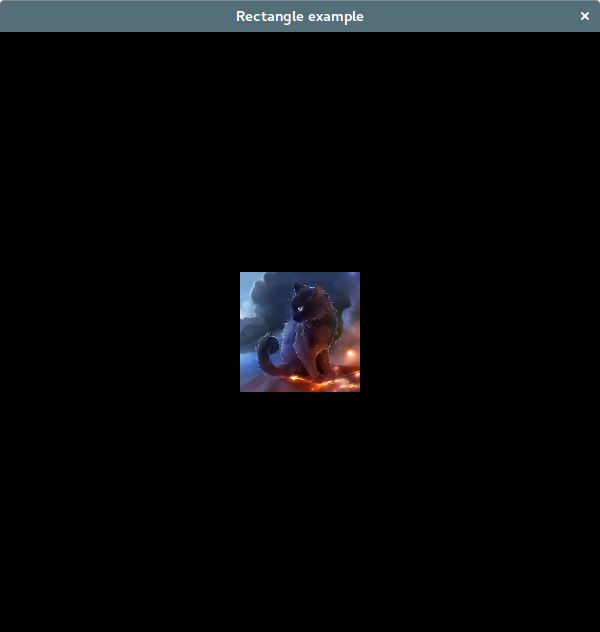
\includegraphics[width=0.7\textwidth]{sprite_example}
    \caption{Sprite example}
    \label{fig:sprite_example}
\end{figure}
